% =====================================================================
%  Accessly – Kraków without barriers · HackYeah 2026 pitch deck (English)
%  Same structure as main.tex (Polish); at most 10 slides (competition rule).
%  One slide = one file in slides-en/. Screenshots with the English interface
%  are in img-en/ (logo and other shared images fall back to img/).
%
%  Build:  latexmk main-en.tex (XeLaTeX, Atkinson Hyperlegible from fonts/)   |   ./build.sh --en [--docker] [--notes]
%          latexmk -pdf main-en.tex: pdfLaTeX fallback with Latin Modern
% =====================================================================
\documentclass[aspectratio=169,10pt,t]{beamer}

\usepackage{iftex}
\ifPDFTeX
  \usepackage[utf8]{inputenc}
  \usepackage[T1]{fontenc}
  \usepackage{lmodern}
  \usepackage[english]{babel}
\else
  \usepackage{fontspec}
  \usepackage{polyglossia}
  \setmainlanguage{english}
  % Typefaces (Atkinson Hyperlegible Next and Mono from fonts/) are set by the theme: beamerthemeaccessly.sty.
\fi
\usepackage{graphicx}
\graphicspath{{img-en/}{img/}}
\usepackage{tabularx}
\usepackage{url}
\urlstyle{same}
\usetheme{accessly}

\hypersetup{
  pdftitle={Accessly – Kraków without barriers (HackYeah 2026)},
  pdfauthor={Team Accessly},
  pdfsubject={Prototype of an accessibility guide and barrier map},
  colorlinks=true, urlcolor=accNavy, linkcolor=accInk,
}

% ---------- Fill in before submitting ----------
\newcommand{\TeamName}{Team Accessly}                      % team name
\newcommand{\TeamId}{Team ID: \ldots}                      % HackTribe team ID
\urldef{\DemoUrl}\url{https://accessly.example.pl}         % live demo
\urldef{\RepoUrl}\url{https://github.com/HakerSII/accessly}   % source code
\urldef{\VideoUrl}\url{https://youtu.be/...}               % video (max 3 min, open repository)

\title[Accessly]{Accessly}
\subtitle[Kraków without barriers \textperiodcentered\ HackYeah 2026]{The city. Accessible for you.}
\author{\TeamName}
\date{HackYeah, 3--4 October 2026}

% ./build.sh --en --notes defines \shownotes and appends the speaker notes after every slide.
\ifdefined\shownotes
  \setbeameroption{show notes}
\fi

\begin{document}

% Slide 1 – title. Team name, ID and links are set in main-en.tex.
{
\setbeamercolor{background canvas}{bg=accNavy}
\setbeamercolor{normal text}{fg=white}
\usebeamercolor[fg]{normal text}
\hypersetup{urlcolor=white}   % links on the navy background; outside this group they return to the main.tex colour
\begin{frame}[plain]
  \vspace{6mm}
  \begin{columns}[T,onlytextwidth]
    \begin{column}{0.64\textwidth}
      \begin{tikzpicture}
        \node[fill=white,rounded corners=2.5mm,inner sep=1mm] {
\includegraphics[height=12mm]{logo}};
      \end{tikzpicture}

      \vspace{2mm}
      {\usebeamerfont{title}\color{white}Accessly\par}
      \vspace{0.5mm}
      {\Large\bfseries\color{white}Kraków without barriers\par}
      \vspace{1.5mm}
      {\color{accSignal}The city. Accessible for you.\par}
      \vspace{10mm}
      {\small\color{white}
        \textbf{\TeamName}\ \textperiodcentered\ \TeamId\par
        HackYeah 2026 \textperiodcentered\ “Cracow without barriers” challenge\par
        \vspace{2.5mm}
        {\footnotesize
        Demo: \DemoUrl\\
        Code: \RepoUrl\\
        Video (3~min): \VideoUrl\par}}
    \end{column}
    \begin{column}{0.32\textwidth}
      \centering
      \vspace{-1mm}
      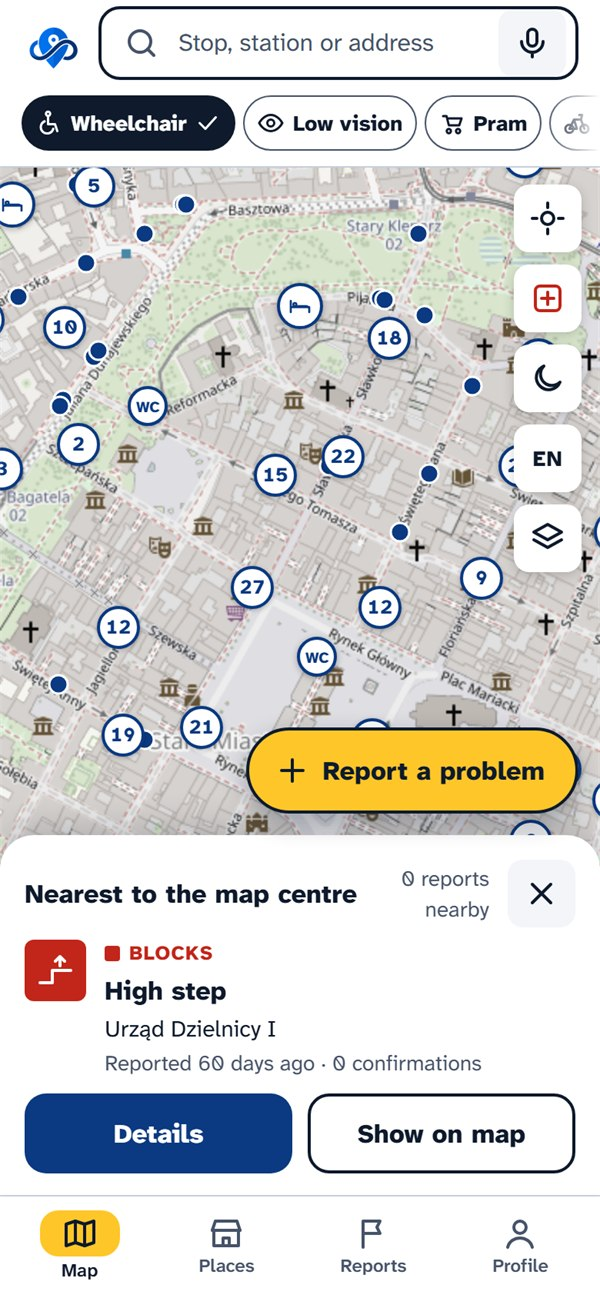
\includegraphics[height=70mm]{mobile-mapa}
    \end{column}
  \end{columns}

  \note[item]{One sentence: Accessly does not say “this place is accessible”; it says “this place will work for you”, and shows where we know it from, since when, and how far it can be trusted.}
  \note[item]{Show the phone next to the laptop: the same prototype runs on both.}
  \note[item]{Do not read the links out loud; they are in the PDF.}
\end{frame}
}

% Slide 2 – problem and target group (criterion: relevance and usefulness for the group, 25 %).
\begin{frame}{Reliable information instead of guesswork}
  \begin{columns}[T,onlytextwidth]
    \begin{column}{0.49\textwidth}
      \begin{block}{Problem}
        \begin{itemize}
          \item Accessibility data is scattered, incomplete and quickly goes out of date.
          \item Without a source and a date, users cannot tell whether to trust it.
          \item Keeping a complete database for a whole city up to date by hand does not scale.
        \end{itemize}
      \end{block}
    \end{column}
    \begin{column}{0.49\textwidth}
      \begin{block}{Who it is for}
        People with access needs and their carers, parents with prams, older people, people recovering from
        medical procedures, tourists with luggage or pets, and the medical tourism industry.
      \end{block}
    \end{column}
  \end{columns}
  \vspace{1mm}
  \begin{exampleblock}{Accessly}
    Combines public data, information from venue owners and confirmations from the community.\\
    Every piece of information has a source, a date and a verification status.
  \end{exampleblock}

  \note[item]{Open with the story: Anna, a wheelchair user, wants a coffee in the centre. Last year's map says “accessible”; today there is a step at the door and nobody knows whether the toilet is downstairs.}
  \note[item]{Primary group from the brief: wheelchairs and prams (the “Wheelchair” and “Pram” profiles). The other profiles reuse the same attributes, so they cost nothing extra.}
  \note[item]{Stress the two groups: end users and owners; without owners the data will not stay current.}
  \note[item]{A profile is a set of preferences (steps, lift, quiet), not disability information; this comes back on the privacy slide.}
\end{frame}

% Slide 3 – what the prototype already does (criterion: quality and completeness of the prototype, 20 %).
\begin{frame}{A working prototype: a web app for phone and desktop}
  \begin{columns}[T,onlytextwidth]
    \begin{column}{0.57\textwidth}
      \small
      \begin{itemize}
        \setlength{\itemsep}{2.5mm}
        \item \textbf{6,545 places, 27 accessibility features}\\
              Concrete information about the entrance, lift, toilet, parking and other needs.
        \item \textbf{Matched to the user}\\
              The needs profile filters and ranks places by what really matters.
        \item \textbf{Live, trustworthy data}\\
              Source, date and verification status for every piece of information, plus community confirmations.
        \item \textbf{AI + barrier map}\\
              The assistant recommends places, and users report and update real obstacles.
      \end{itemize}
    \end{column}
    \begin{column}{0.41\textwidth}
      \screenshot{mapa-desktop}
      \vspace{0.3mm}
      \muted{“Wheelchair” profile: places, layers, reported barriers with severity and confirmations.
        The list next to the map is its text alternative.}
      \vspace{1.5mm}

      \kpi{6,545}{places from OSM}\hfill\kpi{11}{data layers}\hfill\kpi{503}{tests, offline}
    \end{column}
  \end{columns}

  \note[item]{This is not a mock-up: everything on the slide runs from the repository (Python standard library plus plain JavaScript, no dependencies).}
  \note[item]{Place data from OSM: 1,495 of 6,545 places already have at least one accessibility attribute; the rest show “No data”, and that is exactly what we display.}
  \note[item]{Layers: stops with platform kerb type, toilets, disabled parking, lifts, kerbs, crossings with tactile paving, bike routes and infrastructure, luggage storage, A\&E and 24-hour pharmacies.}
  \note[item]{The AI assistant is optional; the demo container runs the keyword mode, so nothing depends on the network.}
\end{frame}

% Slide 4 – map of the live demo (brief, section 6: define the group's needs, check a place, show concrete
% barriers and facilities, the source and date of each fact, how incomplete and sample data are marked).
% The slide stays on screen just before switching to the app; details are in the notes.
\begin{frame}{Demo: Karolina plans a trip to a café}
  \begin{columns}[T,onlytextwidth]
    \begin{column}{0.63\textwidth}
      \small
      Karolina is planning to go to a café with someone close to her who uses a wheelchair.

      \vspace{0.5mm}
      \begin{enumerate}
        \setlength{\itemsep}{0.4mm}
        \item \textbf{She sets the needs}\\
              Wheelchair + step-free entrance + accessible toilet
        \item \textbf{Accessly suggests places}\\
              A ranking of cafés matched to the profile, showing:
              \begin{itemize}
                \setlength{\itemsep}{0pt}\setlength{\topsep}{0pt}
                \item what is accessible,
                \item what is missing,
                \item how up to date the data is.
              \end{itemize}
        \item \textbf{She checks the details}\\
              Next to every fact she sees: source \textperiodcentered\ date \textperiodcentered\ verification status
        \item \textbf{She decides}\\
              She picks a place she can trust -- before they leave home.
      \end{enumerate}
    \end{column}
    \begin{column}{0.34\textwidth}
      \screenshot{karta-dopasowanie}\par
      \vspace{0.3mm}
      \muted{Step 2: what the place meets, what is missing, what is unknown.}
      \vspace{1.5mm}
      \screenshot{karta-atrybut}\par
      \vspace{0.3mm}
      \muted{Step 3: value, source (OpenStreetMap), date (2~Oct 2026) and verification status.}
    \end{column}
  \end{columns}

  \vfill
  {\centering\color{accNavy}\bfseries
    Accessly helps carers plan an outing without guesswork or stress on arrival.\par}
  \vspace{1mm}

  \note[item]{Time: about 3 minutes. Before going on stage: the app open on a phone and a laptop, the “Wheelchair” profile selected, the map on the Main Square (zoom 16), the owner panel open in a second browser tab.}
  \note[item]{Step 1 (0:00–0:30): tap the “Wheelchair” chip; show the toast with the report count and the “Nearest to the map centre” list.}
  \note[item]{Step 2 (0:30–1:00): Places tab, type “A café in the centre I can enter in a wheelchair, ideally with an accessible toilet”; in keyword mode the result is deterministic. Read out what it meets and what is “No data”.}
  \note[item]{Step 3 (1:00–1:45): open the card; point at three things next to the attribute: source, date, status. Then “No data”: our most important message, we do not guess. Buttons Up to date / Outdated / Correct, “Add” and a question to the owner.}
  \note[item]{Step 4 (1:45–2:20): “Report a problem”, pin at the stop, type “No lift”, severity “Blocks”; show the marker shape (square = blocks) and the votes. A report needs no account.}
  \note[item]{Step 5 (2:20–3:00): in the second tab, \texttt{/owner.html} as \texttt{kasia@accessly.test} (Camelot Cafe), click “Potwierdź informacje” (the owner panel is in Polish, for venue staff; say what the button does: confirm the information); back on the card the status has changed.}
  \note[item]{Edge cases (if the jury asks or time is left): attribute history with conflicting votes; the “Data sources” page with snapshot dates; a place with a missing attribute does not get the “Matches your needs” badge.}
  \note[item]{If the network fails: everything except the map tiles works from local data. Sample data: three demo accounts and test reports; the admin view without sign-in carries a “Demo mode: sample data” label.}
\end{frame}

% Slide 5 – data sources, freshness, trustworthiness (criterion: reliability, presentation and updating of data, 15 %).
\begin{frame}{Data you can trust}
  \begin{columns}[T,onlytextwidth]
    \begin{column}{0.49\textwidth}
      \begin{block}{3 sources of information}
        \begin{itemize}
          \setlength{\itemsep}{0.3mm}
          \item \textbf{Open Data \& OSM}\\
                Public and open data
          \item \textbf{Property Owner}\\
                Confirmed information straight from the venue owner
          \item \textbf{Community}\\
                Users confirm, correct and complete the data
        \end{itemize}
      \end{block}
    \end{column}
    \begin{column}{0.49\textwidth}
      \begin{block}{Every fact has context}
        \centering\textbf{Source \textperiodcentered\ Date \textperiodcentered\ Verification status}\par
      \end{block}
      \vspace{1mm}
      \begin{exampleblock}{Accessly Trust Model}
        \pill{accNavy}{Owner verified} $\rightarrow$ \pill{accOk}{Community confirmed} $\rightarrow$\\[0.8mm]
        \pill{accNavy}{Official source} $\rightarrow$ \pill{accMuted}{Unverified}
        \begin{itemize}
          \setlength{\itemsep}{0pt}
          \item outdated data is flagged,
          \item conflicts are visible,
          \item missing information never means “accessible”.
        \end{itemize}
      \end{exampleblock}
    \end{column}
  \end{columns}

  \note[item]{Test case required by the brief -- conflicting data: the owner says “step-free”, two people report “outdated” $\rightarrow$ status “Needs re-checking”, the value stays with a warning, both sides are visible in the history.}
  \note[item]{Case -- source unavailable: the city's ArcGIS service does not respond $\rightarrow$ the app shows the layer from the snapshot with an “as of” date; no screen is ever empty.}
  \note[item]{Case -- incomplete data: “Meets 1 of 3 of your needs, no data: wide doors” -- the place does not get the “Matches your needs” badge.}
  \note[item]{We also checked Kraków's GTFS feeds and dane.gov.pl: their accessibility fields are empty and nobody publishes lift outages, which is why outages come from user reports.}
\end{frame}

% Slide 6 – architecture and scaling (criteria: deployment potential and scalability, 20 %; RULES: Design / Technical).
\begin{frame}{Architecture: data acquisition separated from presentation}
  \centering
  \begin{tikzpicture}[x=1mm,y=1.32mm,
      box/.style={draw=accLineStrong,fill=accSoft,rounded corners=1.2mm,text width=23mm,align=center,
                  font=\fontsize{6.3}{7.6}\selectfont,execute at begin node={\hyphenpenalty=10000},
                  inner sep=1mm,minimum height=8.5mm},
      tall/.style={box,minimum height=42mm},
      head/.style={font=\scriptsize\bfseries,text=accNavy,anchor=south},
      ext/.style={draw=accLineStrong,dashed,fill=white,rounded corners=1.2mm,text width=142mm,align=center,
                  font=\fontsize{6.3}{7.6}\selectfont,execute at begin node={\hyphenpenalty=10000},
                  inner sep=1.2mm},
      arr/.style={-{Stealth[length=1.5mm]},accNavy,line width=0.5pt},
      both/.style={{Stealth[length=1.5mm]}-{Stealth[length=1.5mm]},accNavy,line width=0.5pt}]
    % column headers
    \node[head] at (12.5,46.5) {SOURCES};
    \node[head] at (42,46.5) {ACQUISITION AND UPDATES};
    \node[head] at (72,46.5) {STORAGE};
    \node[head] at (102,46.5) {JSON API};
    \node[head] at (131.5,46.5) {PRESENTATION};
    % column 1: sources
    \node[box] (s1) at (12.5,42) {OpenStreetMap (ODbL)};
    \node[box] (s2) at (12.5,33.5) {Kraków open data (ArcGIS)};
    \node[box] (s3) at (12.5,25) {Venue owners};
    \node[box] (s4) at (12.5,16.5) {Community: confirmations, corrections, barrier reports};
    % column 2: acquisition
    \node[box] (i1) at (42,42) {\texttt{build\_osm\_*.py} $\rightarrow$ snapshots in \texttt{data/}};
    \node[box,minimum height=8mm] (i2) at (42,33) {\texttt{layers.py}: paged fetching, 24-hour cache, background refresh};
    \node[box,minimum height=12mm] (i3) at (42,20.5) {\texttt{api.py}: owner changes, corrections and votes, moderation; every change goes to the history};
    % column 3: storage
    \node[tall] (db) at (72,29) {\textbf{SQLite} (standard library)\\[0.8mm]places \textperiodcentered\ attributes: value, source, date, confirmations, disputes \textperiodcentered\ history \textperiodcentered\ barrier reports and votes \textperiodcentered\ accounts and roles \textperiodcentered\ photos\\[0.8mm]versioned migrations, WAL, transactions};
    % column 4: API
    \node[tall] (api) at (102,29) {\textbf{\texttt{server.py} / \texttt{api.py}}\\[0.8mm]\texttt{/api/places} (profile $\rightarrow$ match, status)\\\texttt{/api/layers} \textperiodcentered\ \texttt{/api/reports}\\\texttt{/api/ai} \textperiodcentered\ \texttt{/api/route}\\\texttt{/api/owner} \textperiodcentered\ \texttt{/api/admin}\\[0.8mm]size limits, gzip, roles};
    % column 5: presentation
    \node[box] (p1) at (131.5,42) {Web app (phone and desktop), 4~languages};
    \node[box] (p2) at (131.5,33.5) {Owner panel};
    \node[box] (p3) at (131.5,25) {Admin panel};
    \node[box] (p4) at (131.5,16.5) {API clients (planned Open API): city, maps, booking};
    % arrows
    \draw[arr] (s1) -- (i1);
    \draw[arr] (s2) -- (i2);
    \draw[arr] (s3.east) -- (i3.west |- s3.east);
    \draw[arr] (s4.east) -- (i3.west |- s4.east);
    \draw[arr] (i1.east) -- (db.west |- i1.east);
    \draw[arr] (i2.east) -- (db.west |- i2.east);
    \draw[arr] (i3.east) -- (db.west |- i3.east);
    \draw[both] (db) -- (api);
    \draw[both] (api.east |- p1.west) -- (p1.west);
    \draw[both] (api.east |- p2.west) -- (p2.west);
    \draw[both] (api.east |- p3.west) -- (p3.west);
    \draw[arr] (api.east |- p4.west) -- (p4.west);
    % optional services
    \node[ext] at (72,6.5) {\textbf{Optional services, each with a fallback:} Claude API (recommendations; keyword rules without a key) \textperiodcentered\ OpenRouteService (wheelchair routes) \textperiodcentered\ Nominatim (search from the browser, only on submit) \textperiodcentered\ Rampa backend (barrier reports through the \texttt{api.js} adapter)};
  \end{tikzpicture}

  \note[item]{Key sentence: importing and refreshing data is a separate step (scripts, snapshots, cache), and the presentation reads only from the database through the API, so the frontend or a source can be swapped without touching the rest.}
  \note[item]{The Rampa backend (FastAPI, PostgreSQL, observation $\rightarrow$ vote $\rightarrow$ trust model) was built in parallel; the adapter in \texttt{api.js} moves barrier reports there without changes to the app. That is the scaling path for a larger deployment.}
  \note[item]{Honestly: the city layer configuration lives in code today (\texttt{layers.py}), not in the city file; that is the first step for a second city.}
\end{frame}

% Slide 7 – digital accessibility (brief, sections 5–6: WCAG 2.2 AA target, list of features and gaps).
% Cards and icons: \accesscard in beamerthemeaccessly.sty.
\begin{frame}{Accessible from day one}{Goal: WCAG 2.2 AA}
  \vspace{2mm}
  \centering
  \begin{tikzpicture}[x=1mm,y=1mm]
    % Section 1: already working (3 × 2 grid)
    \node[anchor=south west,inner sep=0pt,font=\small\bfseries,text=accOk] at (0,0.5) {Already working};
    \accesscard{14.75}{-11.5}{keyboard}{Keyboard navigation}
    \accesscard{46.75}{-11.5}{speaker}{Screen readers}
    \accesscard{78.75}{-11.5}{listlines}{Text alternative to the map}
    \accesscard{14.75}{-32.5}{contrast}{Contrast and legibility}
    \accesscard{46.75}{-32.5}{zoom}{Large touch targets + 400\,\% zoom}
    \accesscard{78.75}{-32.5}{bubble}{4~languages}

    % Section 2: next step
    \node[anchor=south west,inner sep=0pt,font=\small\bfseries,text=accPartial] at (100,0.5) {Next step};
    \draw[nextpanel] (100,-2) rectangle (144,-42);
    \node[anchor=north west,text width=38mm,inner sep=0pt,font=\small,text=accInk] at (103,-7.5) {%
      \begin{itemize}
        \setlength{\itemsep}{3mm}
        \item User testing
        \item NVDA / VoiceOver audit
        \item Full compliance of the Owner / Admin panels
      \end{itemize}};

    % Strong closing statement
    \node[font=\normalsize\bfseries,text=accNavy] at (72,-49.5)
      {Accessibility is not an add-on -- it is part of Accessly's architecture.};
  \end{tikzpicture}

  \note[item]{Show live: Tab through the reports list, Enter opens the details, Esc goes back; switch to night mode.}
  \note[item]{A “text alternative to the map” is an explicit requirement of the brief; for us the list next to the map is a first-class view, not an add-on.}
  \note[item]{Contrast: a test computes the ratios from the tokens in \texttt{style.css} for both themes; separators have their own token, control borders and layer symbols have 3:1.}
  \note[item]{Do not say “we are WCAG compliant”; say “the main scenario meets the A/AA criteria we checked, and here is the list of gaps”.}
\end{frame}

% Slide 8 – data protection and security, running and maintaining the service outside the City Hall (brief, section 5).
% Two cards with icon + text rows: \inforow and the icons in beamerthemeaccessly.sty.
\begin{frame}{Privacy and simple operations}
  \vspace{3mm}
  \centering
  \begin{tikzpicture}[x=1mm,y=1mm]
    % Card 1: privacy by design
    \fill[infocard] (0,0) rectangle (70,-46);
    \node[anchor=north west,inner sep=0pt,font=\normalsize\bfseries,text=accNavy] at (5,-4) {Privacy by design};
    \inforow{8.5}{-14}{person}{Use without an account, anonymous reports}
    \inforow{8.5}{-23}{listlines}{Needs profile without medical data or diagnoses}
    \inforow{8.5}{-32}{key}{Secure passwordless sign-in}
    \inforow{8.5}{-40.5}{lock}{HTTPS, roles and access control}

    % Card 2: easy deployment and operations
    \fill[infocard] (74,0) rectangle (144,-46);
    \node[anchor=north west,inner sep=0pt,font=\normalsize\bfseries,text=accNavy] at (79,-4) {Easy to deploy and run};
    \inforow{82.5}{-13}{cloud}{Runs outside City Hall infrastructure}
    \inforow{82.5}{-20.2}{refresh}{Automatic data updates}
    \inforow{82.5}{-27.4}{box}{Docker -- deploy on any VPS}
    \inforow{82.5}{-34.6}{coin}{Hosting: approx.\ PLN~60--120 / month}
    \inforow{82.5}{-41.8}{shieldcheck}{Moderation in the admin panel}

    % Strong closing statement
    \node[font=\normalsize\bfseries,text=accNavy,text width=144mm,align=center,inner sep=0pt] at (72,-52.5)
      {Minimum user data. Minimum running costs. Maximum portability.};
  \end{tikzpicture}

  \note[item]{Jury question “what data do you collect?”: without an account, none; with an account, e-mail, an optional display name and the needs profile. The table is in the privacy policy inside the app.}
  \note[item]{GDPR: the needs profile is a deliberate design decision; the brief explicitly asks not to require disability information.}
  \note[item]{The amounts are estimates from VPS price lists; do not promise a specific provider.}
\end{frame}

% Slide 9 – business model and commercialisation (criterion: 20 %; brief, section 9).
% Four cards, 2 × 2: \bizcard and the icons in beamerthemeaccessly.sty; the yellow label is the revenue source.
\begin{frame}{How does Accessly make money?}
  \vspace{1mm}
  \centering
  \begin{tikzpicture}[x=1mm,y=1mm]
    \bizcard{0}{0}{house}{Property Owner Pro}{Hotels, restaurants, galleries, chains}
      {Subscription per venue / package for chains}
      {\bp\mbox{statistics on users' needs} \quad \bp\mbox{accessibility widget} \quad \bp\mbox{managing many locations}}
    \bizcard{73}{0}{cityskyline}{Cities and regions}{}
      {White-label + maintenance}
      {\bp\mbox{local data and city layers} \quad \bp\mbox{reports on barriers and gaps} \quad \bp\mbox{fast roll-out to further cities}}
    \bizcard{0}{-29.5}{apicode}{API \& partners}{Maps, booking, travel apps}
      {API licence / subscription}
      {\bp\mbox{verified accessibility data} \quad \bp\mbox{integrations with booking systems}}
    \bizcard{73}{-29.5}{medcross}{Medical tourism}{Clinics, hotels, stay operators}
      {B2B packages / integrations}
      {\bp\mbox{clinic + stay + transport + services} \quad \bp\mbox{recommendations for patients and carers}}

    \node[font=\small\bfseries,text=accNavy,text width=144mm,align=center,inner sep=0pt] at (72,-61.8)
      {Users pay nothing. Businesses pay for tools, integrations and analytics --\\
       never for a better accessibility status.};
  \end{tikzpicture}

  \note[item]{The most realistic first revenue: hotels and medical tourism (the “After treatment” profile, the A\&E / pharmacies layer, 4~languages); guests from abroad ask about accessibility before booking.}
  \note[item]{The owner panel already shows “the most searched-for information about your venue”; that is the seed of the Pro plan statistics.}
  \note[item]{Event package: the owner panel already has bulk-added points inside a venue (lifts, toilets, entrances); an organiser adds them for the duration of the event.}
  \note[item]{The city is not the first customer; it uses the data and the reports, and may fund a white-label deployment.}
\end{frame}

% Slide 10 – from prototype to service: what exists, what comes next, closing sentence (brief, section 6).
% Two columns (We have today / Next step) with a “Today → Pilot → Scale” arrow, then a navy mission band and the tagline.
\begin{frame}{From prototype to service}
  \centering
  \begin{tikzpicture}[x=1mm,y=1mm,
      col/.style={anchor=north west,text width=66mm,inner sep=0pt,font=\small,text=accInk,align=flush left,
                  execute at begin node={\hyphenpenalty=10000}},
      stage/.style={rounded corners=2.2mm,minimum height=5.2mm,inner xsep=3mm,font=\scriptsize\bfseries}]
    % Stages
    \node[stage,fill=accOk,text=white,anchor=west] (s1) at (0,1) {Today};
    \node[stage,fill=accNavy,text=white,anchor=west] (s2) at (78,1) {Pilot};
    \node[stage,draw=accNavy,text=accNavy,fill=white,anchor=east] (s3) at (144,1) {Scale};
    \draw[flow] (s1.east) -- (s2.west);
    \draw[flow] (s2.east) -- (s3.west);

    % We have today
    \node[col,text width=74mm] at (0,-4) {%
      {\normalsize\bfseries\color{accOk}We have today\par}\vspace{1.2mm}
      \begin{itemize}\setlength{\itemsep}{0.3mm}
        \item 6,545 places and 27 accessibility features
        \item source, date and verification status for every piece of information
        \item Open Data + Property Owner + Community
        \item barrier map, AI, 4~languages and a working prototype
      \end{itemize}};

    % Next step
    \node[col] at (78,-4) {%
      {\normalsize\bfseries\color{accNavy}Next step\par}\vspace{1.2mm}
      \begin{itemize}\setlength{\itemsep}{0.3mm}
        \item pilot with users and partners
        \item integrations with hotels, clinics and booking systems
        \item Open API and more cities
      \end{itemize}};

    % Mission: the strongest element of the slide
    \fill[accNavy,rounded corners=3mm] (0,-37) rectangle (144,-50);
    \node[text width=136mm,align=center,inner sep=0pt,text=white,font=\large\bfseries,
          execute at begin node={\hyphenpenalty=10000}] at (72,-43.5)
      {Reliable, up-to-date and verifiable accessibility information --
       before they arrive.};

    % Final tagline
    \node[inner sep=0pt,font=\Large\bfseries] at (72,-56.5)
      {\raisebox{-0.36\height}{
\includegraphics[height=12mm]{logo}}\hspace{1.5mm}{\color{accNavy}Accessly} {\color{accMuted}--} {\color{accInk}accessibility information you can trust.}};
  \end{tikzpicture}

  \note[item]{Close with the sentence in the navy band and invite the jury to the table with the phone: let them tap “Report a problem” themselves.}
  \note[item]{Question about the team after the hackathon: an operator (company / foundation), moderation in the panel, funding from the Pro plan and white-label deployments.}
  \note[item]{Question about a second city: it needs a name and bounds (the city file), an OSM extract from Geofabrik and, if the city has them, open layers (stops, toilets, parking). Without city data, OSM alone works.}
  \note[item]{The links (demo, code, video) are on the title slide.}
\end{frame}


\end{document}
